%!TEX program = xelatex.exe
\documentclass[14pt,a4paper]{article}
\usepackage{cmap} %Улучшает поиск по pdf документу
\usepackage[pdftex,
    pdfauthor={К.С.~Пилипенко},
    pdftitle={Лекции по радиологии},
    pdfsubject={The Subject},
    pdfkeywords={Первое ключевое слово, второе ключевое слово},
    pdfproducer={LuaLatex with hyperref},
    pdfcreator={Lualatex},
    hidelinks
]{hyperref}
%%%%%%%%%%%%%%Пользовательские команды%%%%%%%%%
\usepackage{latexsym,amsmath,amssymb,amsbsy,graphicx}
\usepackage{tikz}
\usetikzlibrary{shapes,arrows}
\tikzstyle{block} =
        [
                rectangle,
                % draw,
                fill = teal!10,
                % text width = 6em,
                text centered,
                rounded corners,
                node distance = 3 cm,
                minimum height = 2em
        ]
\tikzstyle{line} =
        [
                very thick,
                draw=teal!10,
                -latex'
        ]
\usepackage{icomma}
\usepackage[version=4]{mhchem} % the canonical chemistry package (example: \ce{^{32}_{15}P})
\usepackage{csquotes}
\usepackage{graphicx}
\graphicspath{{images/}}
\DeclareGraphicsExtensions{.pdf,.png,.jpg}
%%%%%%%%%%%%%%%%%%%%%%%%Оформление по ГОСТУ
\usepackage{fontspec}
\setmainfont[Renderer=Basic,Ligatures={TeX}]{Times New Roman}
\usepackage[english,russian]{babel} %Поддержка русской локализации
\usepackage[14pt]{extsizes} % для того чтобы задать нестандартный 14-ый размер шрифта
\usepackage{indentfirst} %Задаёт отступ самого первого абзаца
\setlength\parindent{1.25cm}
\usepackage[a4paper, left=3cm, top=1.5cm, right=1.5cm, bottom=2cm]{geometry}
\usepackage{setspace}
\usepackage[version=4]{mhchem} % the canonical chemistry package(example: \ce{^{32}_{15}P})
%\sloppy %Выравнивание текст по ширине и решение проблемы переполнением строки
\onehalfspacing %Полуторный интервал
\usepackage{mathtext} % русские буквы в формулах
\usepackage{caption} %заголовки плавающих объектов
\captionsetup[figure]{name=Рис.} % меняет название рисунков на русское
%%%%%%%%%%%%%%%%%%%%%%%%%%%%%
\title{Лекции по радиологии}
\author{\href{mailto:www-kirill.pilipenko@yandex.ru}{К.С.~Пилипенко}} %Через \and можно добавить ещё авторов
\date{\selectlanguage{russian}\today}
\begin{document}
\maketitle
\section{Основные понятия радиологии}
\textbf{Радиология}~---~это раздел медицины, изучающий применение лучевых методов для диагностики  и лечения различных заболеваний, а также заболевания и патологические состояния, возникающие при воздействии ионизирующих излучений на организм человека.
Радиологию делят на: \textit{лучевую диагностику (диагностическую радиологию) и лучевую
терапию (радиационную терапию)}.

\textbf{Лучевая диагностика}~---~наука о применении излучений для исследования строения и функций нормальных и патологически измененных органов и систем человека с целью профилактики и распознавания заболеваний. Подразделяется на: 
\begin{enumerate}
    \item рентгенодиагностика; 
    \item радионуклидная диагностика;
    \item ультразвуковая диагностика;
    \item магнитно-резонансная визуализация;
    \item интервенционная радиология: выполнение лечебных вмешательств под контролем лучевых исследований
\end{enumerate}
Также к радиологии относят термографию, СВЧ-термометрию и магнитно-резонансную спектрометрию.

\textbf{Лучевая терапия}~---~это наука о применении ионизирующих излучений для лечения болезней. Делят по типу излучения на: 1) квантовое; 2) корпускулярное.

\textbf{Радиационная биология}~---~наука, которая изучает действие ионизирующих излучений на живые объекты.

Смежные дисциплины радиологии:
\begin{itemize}
    \item кардиология;
    \item пульмонологию; 
    \item остеопатология; 
    \item гастроэнтерология; 
    \item эндокринология и др.
\end{itemize}

\section{История формирования радиологии}
День рождения радиологии --- \emph{8 ноября 1895 г}. Вечером этого дня в баварском городе Вюрцбурге, в физической лаборатории местного университета профессор Вильгельм Конрад Рентген, работая с катодной трубкой, случайно заметил свечение, исходившее от банки с кристаллами платиносинеродистого бария. Рентген настолько полно изучил новое излучение, что до 1908 г. к установленным им данным не было добавлено ничего существенного.
\begin{center}
    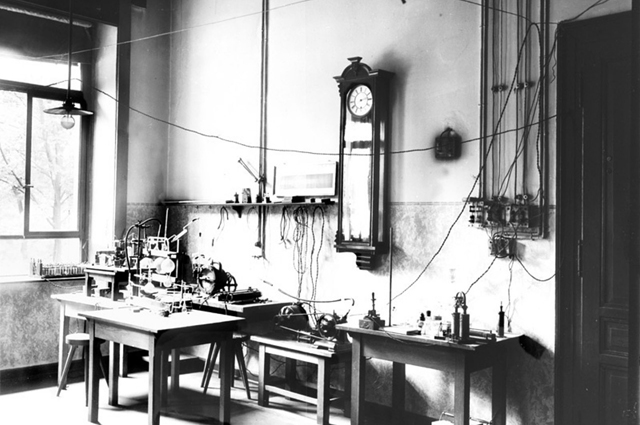
\includegraphics[width=.4\textwidth]{RentgenLab}
\end{center}

Забавно, но первоначально Рентген прислал рождественские поздравления со снимком кисти своей руки перед тем, как обнародовать своё открытие.

Стокгольм, \emph{10 декабря 1903 г}. В зале Шведской академии наук, на том
месте, где 2 года назад стоял Рентген, находился невысокий человек, тоже
физик, но из Франции — Анри Беккерель. Открытие явления естественной радиоактивности.

Супруги Кюри работали непрерывно в течении 2 лет и переработав около 7 т руды, они получили
около 1 г нового элемента, который оказался в 1 млн раз активнее урана.
Этот элемент был назван ими «радий», что в переводе на русский язык означает «лучистый». Затем ими был открыт элемент, испускавший еще более интенсивное излучение, чем уран (в 10 млрд раз).
Он был назван полонием в честь Польши — родины М. Склодовской-Кюри.

В 30-е годы американский физик Э.Лоуренс предложил использовать ускорение элементарных частиц для придания им высоких энергий. Вскоре Э. Лоуренс воплотил эту идею в жизнь, построив циклотрон. Циклотрон стал одним из основных источников получения искусственных радиоактивных элементов и генерации электромагнитных излучений высоких энергий. Появились даже специальные циклотроны медицинского назначения.

\subsection{Рождение отечественной радиологии}
12 января 1896 г. в Петербургском университете были сделаны первые
снимки кисти. 16 января Н.Г. Егоров произвел аналогичный снимок в Медико-хирургической академии, а П.Н. Лебедев — на кафедре физики Московского университета. Одновременно Александр Степанович Попов — изобретатель радио —
изготовил первую в России рентгеновскую установку и выполнил исследование раненного дробью.

в самом начале XX века в России не было условий для развития медицинской радиологии: электротехнической промышленности практически не существовало. Рентгеновские кабинеты были оснащены примитивным оборудованием, причем меры зашиты от излучения не применялись. Во всей стране было лишь несколько десятков врачей-рентгенологов.
Становление медицинской радиологии как самостоятельной научной и
клинической дисциплины произошло только после первой мировой войны.
Радиологи рассматривают это как второе ее рождение.

В 1919 г. в Институте усовершенствования врачей в Петрограде была учреждена первая
кафедра рентгенологии, которую возглавил А.К. Яновский. С 1920 г. стал
выходить журнал «Вестник рентгенологии и радиологии». В последующие
годы были организованы институты рентгенологии в Москве, Киеве, Харь-
кове, Одессе, Ереване, Тбилиси и других городах, созданы заводы рентгено-
аппаратостроения.
\section{Ионизирующее излучение}
\emph{Ионизирующим излучением} (проникающей радиацией, ИИ) называют
высокочастотные электромагнитные излучения энергетических фотонов, которые
превышает величину потенциала ионизации больше, чем 10 эВ ($1\;\text{эВ} = 1,6 \cdot 10^{-19}\;\text{Дж}$). К ИИ относятся рентгеновское излучение и гамма-излучение.

\[ E = 10\;\text{эВ} = 1,6 \cdot 10^{-18}\;\text{Дж}\]
\[ \gamma = \frac{hc}{E} = \frac{6,6\cdot 10^{-34} \cdot 3 \cdot 10^8}{1,6 \cdot 10^{-19}} = 1,2 \cdot 10^{-7}\;\text{м} = 120\;\text{нм}\]
Рентгеновское излучение и гамма-излучение отличаются по энергии, длине
волны и по происхождению.

Получают рентгеновское излучение, как правило, с помощью рентгеновских трубок. Например, при максимальном напряжении 50 киловольт (кВ) средняя энергия рентгеновских квантов около
30 кэВ, при 100 кВ — 65 кэВ, при 150 кВ — 100 кэВ. Рентгеновское излучение именно в данном диапазоне энергий используют в рентгенодиагностике.

\begin{tikzpicture}
    \node [block] (x-ray) {Рентгеновское излучение};
    \node [block, below left of = x-ray] (braking) {Тормозное};
    \node [block, below right of = x-ray] (characteristic) {Характеристическое};
     \path [line] (x-ray) -- (braking);
     \path [line] (x-ray) -- (characteristic);
\end{tikzpicture}

\emph{Тормозное} возникает при торможении заряженных частиц при большом
ускорении. Энергетический спектр является непрерывным.

\emph{Характеристическое} возникает при переходах между далеко расположенными
энергетическими уровнями. Спектр излучения дискретный.

\begin{tikzpicture}
    \node [block] (x-ray) {Рентгеновское излучение по энергии фотона};
    \node [block, below left of = x-ray] (soft) {Мягкое ($E_\text{ф} < 50\;\text{кэВ}$,\\ $\lambda > 25\;\text{нм}$)};
    \node [block, below right of = x-ray] (hard) {Жесткое ($E_\text{ф} > 50\;\text{кэВ}$,\\ $\lambda < 25\;\text{нм}$)};
     \path [line] (x-ray) -- (soft);
     \path [line] (x-ray) -- (hard);
\end{tikzpicture}

\emph{Гамма-излучение} возникает либо при ядерных реакциях, либо при переходах в
энергетических уровнях в ядрах. Энергия
γ-квантов находится в пределах от десятков кэВ до десятков МэВ, поэтому они характеризуются высокой проникающей способностью и выраженным биологическим действием.

К ИИ также относятся: корпускулярные излучения, а именно: $\beta$-частицы, т.е. электроны, позитроны, протоны, $\alpha$-частицы, так же нейтроны и др. частицы.

\emph{Альфа-частица (\ce{^4_2He})} — как бы голое ядро атома гелия, состоящее из
двух протонов (р) и двух нейтронов (n). Следовательно, она имеет двойной
положительный заряд и относительно большую массу, равную 4 атомным
единицам массы. Эта частица возникает при α-распаде естественных радиоактивных элементов. В тканях человеческого тела α-частицы пробегают
лишь несколько десятков микрон.

\emph{Бета-частица} — это либо электрон ($e^{-1}$), либо позитрон ($e^{+1}$). Каждая
β-частица обладает одним элементарным электрическим зарядом: электрон — отрицательным, позитрон — положительным. Масса β-частицы невелика, всего $1/1840$ массы ядра атома водорода. Позитроны образуются при распаде некоторых искусственных радионуклидов. Электроны могут возникать при распаде радионуклидов. В этом случае энергетический спектр β-излучения непрерывный с максимумом до 2 МэВ. В мягких тканях человека такие
электроны распространяются всего на несколько миллиметров. С другой
стороны, электроны могут быть получены в ускорителях заряженных частиц в результате термоэлектронной эмиссии. Такие электроны не принято называть β-частицами. Их энергия может достигать 50 -- 100 МэВ, и они обладают большим пробегом в тканях.

Источники $\alpha-, \beta$-частиц и $\gamma$-лучей естественные радионуклиды такие как: уран; радий; торий;  актиний; радон.

\begin{displayquote}
    В апреле 1902 г. Беккерель по просьбе Пьера Кюри подготовил препарат радия для демонстрации его свойств на конференции. Он положил
    стеклянную трубочку с радием в карман жилета, где она находилась почти
    6 ч Спустя 10 дней на коже под карманом появилась эритема, а еще через
    несколько дней образовалась язва, которая долго не заживала. Встретив-
    шись с Пьером и Марией Кюри, Беккерель сказал: «Я очень люблю радий,
    но я на него в обиде».
\end{displayquote}

\subsection{Не ионизирующее излучение}
В радиологии к неионизирующем излучению относят:
\begin{enumerate}
    \item тепловое (инфракрасное — ИК) излучение;
    \item резонансное, возникающее в объекте (тело
    человека), помещенном в стабильное магнитное поле, под действием высокочастотных электромагнитных импульсов;
    \item условно относят ультразвуковые волны.
\end{enumerate}
\emph{Инфракрасное излучение} испускают все тела, температура которых выше абсолютного нуля. По длине они занимают промежуточное
положение между видимым светом и радиоволнами. Диапазон ИК-лучей —
от 0,76 до 1000 мкм. Интенсивность ИК-излучения пропорциональна 4-й степени температуры тела. Максимальное
излучение тела человека лежит в области длинноволнового ИК-излучения и составляет в среднем 9,6 мкм. 

\emph{Ультразвук} представляет собой волнообразно распространяющееся колебательное движение частиц упругой среды. В зависимости от частоты колебаний звуковые волны делят на инфразвук — до 20 колебаний в секунду — 20 герц (Гц), собственно звук — от 20 Гц до 20 килогерц (кГц) и ультразвук — свыше 20 кГц. В медицинской диагностике применяют ультразвук
частотой от 0,8 до 15 млн герц (МГц).

\subsection{Взаимодействие излучения с веществом}
\end{document}